\chapter{Phương pháp triển khai}

\section{Quy trình tổng thể}


\vspace{10pt}
\begin{figure}[htbp]
\centering
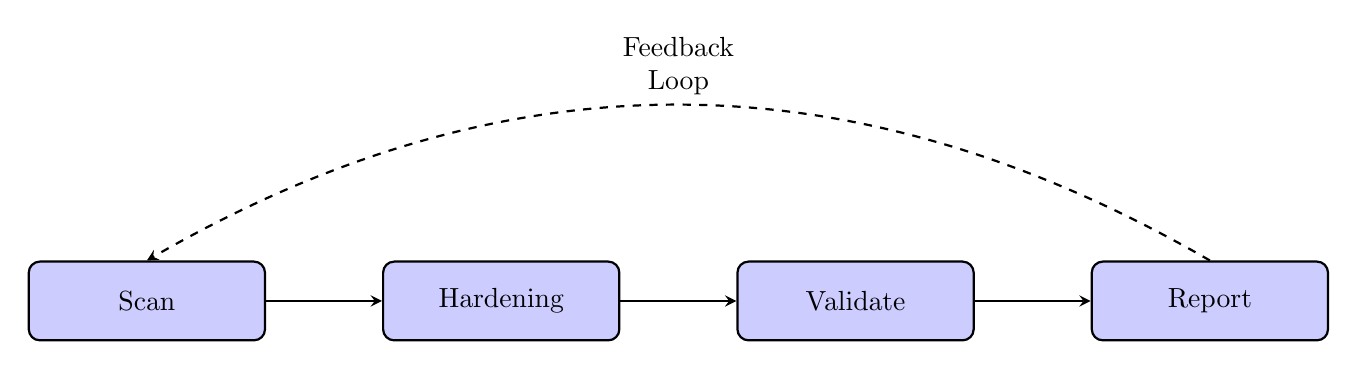
\begin{tikzpicture}[node distance=3.5cm, auto]
    % Define styles
    \tikzstyle{process} = [rectangle, rounded corners, minimum width=3cm, minimum height=1cm, text centered, draw=black, fill=blue!20, line width=0.8pt]
    \tikzstyle{arrow} = [thick,->,>=stealth, line width=0.8pt]
    
    % Place nodes
    \node (scan) [process] {Scan};
    \node (hardening) [process, right of=scan, xshift=1cm] {Hardening};
    \node (validate) [process, right of=hardening, xshift=1cm] {Validate};
    \node (report) [process, right of=validate, xshift=1cm] {Report};
    
    % Draw arrows with proper spacing
    \draw [arrow] (scan.east) -- (hardening.west);
    \draw [arrow] (hardening.east) -- (validate.west);
    \draw [arrow] (validate.east) -- (report.west);
    
    % Feedback loop connecting to top of nodes
    \draw [arrow, dashed, bend right=30] (report.north) to node[above, text width=2cm, text centered] {Feedback Loop} (scan.north);
\end{tikzpicture}
\caption{Quy trình 4 bước triển khai bảo mật hệ thống}
\label{fig:security_process}
\end{figure}

\vspace{5pt}
\noindent Quy trình triển khai bảo mật được thiết kế theo chu trình 4 bước chính, đảm bảo tính toàn diện và có thể lặp lại. Mỗi bước có vai trò cụ thể và liên kết chặt chẽ với nhau để tạo ra một hệ thống bảo mật hoàn chỉnh.

\vspace{5pt}
\noindent Quy trình này bắt đầu từ việc đánh giá trạng thái hiện tại, tiếp theo là áp dụng các biện pháp hardening, sau đó xác thực kết quả và cuối cùng là tạo báo cáo chi tiết. Vòng lặp này giúp đảm bảo hệ thống luôn được cập nhật và tuân thủ các tiêu chuẩn bảo mật mới nhất.

\section{Phương pháp tiếp cận}
\subsection{Manual Configuration}
\vspace{5pt}
\noindent Cấu hình thủ công là phương pháp truyền thống trong quản trị hệ thống. Administrator trực tiếp thực hiện các thay đổi trên hệ thống thông qua command line, giao diện đồ họa hoặc file config.

\vspace{5pt}
\noindent \textbf{Các công cụ sử dụng trong cấu hình thủ công:}
\begin{itemize}
\item \textbf{Command Line Tools:} \texttt{ansible-playbook}, \texttt{systemctl}, \texttt{ufw}, \texttt{iptables}, \texttt{nftables},\\
\texttt{chmod}, \texttt{chown}, \texttt{mount}, \texttt{netstat}, \texttt{lynis}, \texttt{aide}, \texttt{auditd}, \texttt{fail2ban}
\item \textbf{Giao diện đồ họa (GUI):} AWX/Tower, Grafana, Webmin, Cockpit
\item \textbf{File cấu hình:} \texttt{/etc/sysctl.conf}, \texttt{/etc/fstab}, \texttt{/etc/ssh/sshd\_config},\\
\texttt{/etc/network/interfaces}, \texttt{/etc/passwd}, \texttt{/etc/shadow}, \texttt{ansible.cfg}, \texttt{inventory/hosts}, \texttt{playbooks/}
\end{itemize}

\vspace{5pt}
\noindent Phương pháp này có ưu điểm là linh hoạt và dễ kiểm soát từng bước, nhưng nhược điểm lớn là tốn nhiều thời gian, dễ xảy ra sai sót, và khó đảm bảo tính nhất quán giữa nhiều hệ thống khác nhau.

\vspace{5pt}
\noindent Đối với các hệ thống quy mô nhỏ, cấu hình thủ công vẫn có thể được áp dụng cho các tác vụ đặc thù yêu cầu sự can thiệp chuyên sâu.

\subsection{Automation bằng Ansible}
\vspace{5pt}
\noindent Ansible là công cụ tự động hóa mạnh mẽ giúp loại bỏ các thao tác thủ công lặp đi lặp lại. Với Ansible, chúng ta có thể định nghĩa toàn bộ quy trình hardening dưới dạng code, đảm bảo tính nhất quán và có thể tái sử dụng.

\vspace{5pt}
\noindent \textbf{Các công cụ sử dụng trong automation bằng Ansible:}
\begin{itemize}
\item \textbf{Ansible Command Line Tools:} \texttt{ansible-playbook}, \texttt{ansible-inventory},\\
\texttt{ansible-vault}, \texttt{ansible-galaxy}, \texttt{ansible-pull}
\item \textbf{Ansible GUI Tools:} AWX/Tower, Ansible Semaphore, Rundeck, Jenkins với Ansible plugin
\item \textbf{Ansible Configuration Files:} \texttt{ansible.cfg}, \texttt{inventory/hosts}, \texttt{playbooks/*.yml},\\
\texttt{roles/*/tasks/main.yml}, \texttt{group\_vars/*}, \texttt{host\_vars/*}, \texttt{vars/*}, \texttt{vault/*}
\end{itemize}

\vspace{5pt}
\noindent Ansible sử dụng YAML để định nghĩa các playbook, giúp administrator dễ dàng đọc, hiểu và chỉnh sửa. Khả năng idempotent của Ansible đảm bảo rằng việc chạy nhiều lần sẽ không gây ra các trạng thái không mong muốn.

\vspace{5pt}
\section{Mô hình triển khai}

\vspace{10pt}
\begin{figure}[htbp]
\centering
\begin{tikzpicture}[
    node distance=4cm and 3cm,
    every node/.style={font=\small},
    controller/.style={
        rectangle, rounded corners,
        minimum width=3cm, minimum height=1.5cm,
        text centered, draw=black, fill=red!20,
        align=center
    },
    worker/.style={
        rectangle, rounded corners,
        minimum width=2.8cm, minimum height=1.5cm,
        text centered, draw=black, fill=blue!20,
        align=center
    },
    arrow/.style={->, very thick}
]

% Nodes
\node (worker1) [worker] {Worker 1\\Ubuntu 22.04};

\node (worker2) [worker, below=1cm of worker1] {Worker 2\\Ubuntu 24.04};

\node (controller) [controller, left=4cm of $(worker1)!0.5!(worker2)$] {Controller\\Arch Linux};

% Arrows
\draw [arrow] (controller.east) -- (worker1.west);
\draw [arrow] (worker1.west) -- (controller.east);

\draw [arrow] (controller.east) -- (worker2.west);
\draw [arrow] (worker2.west) -- (controller.east);

\end{tikzpicture}
\caption{Mô hình triển khai Controller-Workers}
\label{fig:deployment_model}
\end{figure}

\noindent
Hệ thống được triển khai theo mô hình Controller--Workers, trong đó một máy trung tâm (Controller) chịu trách nhiệm điều phối và quản lý cấu hình, trong khi các máy Worker đóng vai trò là các node mục tiêu được cấu hình tự động.

\vspace{5pt}
\noindent \textbf{Cụ thể trong đề tài:}
\begin{itemize}
\item \textbf{Controller:} Arch Linux (chạy Ansible)
\item \textbf{Worker 1:} Ubuntu 22.04
\item \textbf{Worker 2:} Ubuntu 24.04
\end{itemize}

\vspace{5pt}
\noindent Mô hình này cho phép thực hiện quản lý tập trung, đảm bảo tính nhất quán và giảm thiểu sai sót trong quá trình cấu hình hệ thống.

\subsection{Quy trình triển khai tự động}

\noindent Hệ thống được triển khai theo hướng tự động hóa hoàn toàn thông qua Ansible, đảm bảo tính nhất quán và khả năng tái sử dụng. Quy trình tập trung vào việc định nghĩa cấu hình dưới dạng code, cho phép quản lý tập trung và giảm thiểu sai sót thủ công.

\vspace{5pt}
\noindent Mô hình này hỗ trợ việc triển khai trên nhiều hệ thống đồng thời, với khả năng mở rộng và bảo trì dễ dàng thông qua cơ chế kiểm soát phiên bản.

\subsection{Mô hình triển khai Automated Security Hardening System}

\noindent Dựa trên kiến trúc Controller--Workers, hệ thống Automated Security Hardening được thiết kế thành một quy trình tích hợp khép kín gồm ba thành phần cốt lõi: \textit{Auto-VM}, \textit{CIS-Ubuntu} và \textit{Report Module}. 

\vspace{5pt}
\noindent Mô hình này tự động hóa toàn bộ vòng đời bảo mật từ khâu khởi tạo môi trường, áp dụng cấu hình tiêu chuẩn đến đánh giá và tối ưu hóa hệ thống.

\vspace{10pt}
\begin{figure}[htbp]
\centering
\begin{tikzpicture}[
    node distance=5cm and 3cm,
    every node/.style={font=\small},
    component/.style={
        rectangle, rounded corners,
        minimum width=3.5cm, minimum height=2cm,
        text centered, draw=black, 
        align=center, line width=0.8pt
    },
    auto_vm/.style={component, fill=green!20},
    cis_ubuntu/.style={component, fill=blue!20},
    report/.style={component, fill=orange!20},
    arrow/.style={->, very thick, line width=0.8pt},
    feedback/.style={->, very thick, dashed, bend right=45, line width=0.8pt}
]
% Nodes
\node (auto_vm) [auto_vm] {Auto-VM\\Tự động tạo\\máy ảo};
\node (cis_ubuntu) [cis_ubuntu, right=of auto_vm] {CIS-Ubuntu\\Hardening\\bảo mật};
\node (report) [report, right=of cis_ubuntu] {Đánh giá và\\báo cáo};

% Main workflow arrows
\draw [arrow] (auto_vm.east) -- node[above, text width=2cm, text centered] {VM sẵn sàng} (cis_ubuntu.west);
\draw [arrow] (cis_ubuntu.east) -- node[above, text width=2cm, text centered] {Hệ thống hardening} (report.west);

% Feedback loop
\draw [feedback] (report.north) to node[below, text width=2.5cm, text centered] {Phản hồi cải tiến} (auto_vm.north);

% Labels for technologies
\node[below=0.3cm of auto_vm, text width=3.5cm, text centered, font=\tiny] {KVM/QEMU, Ansible, Cloud-init};
\node[below=0.3cm of cis_ubuntu, text width=3.5cm, text centered, font=\tiny] {CIS Ubuntu 24.04 LTS Benchmark};
\node[below=0.3cm of report, text width=3.5cm, text centered, font=\tiny] {Lynis, OpenSCAP};
\end{tikzpicture}
\caption{Mô hình triển khai Automated Security Hardening System với chu trình khép kín}
\label{fig:automated_security_model}
\end{figure}

\vspace{5pt}
\noindent \textbf{1. Auto-VM (Khởi tạo môi trường)}
\vspace{5pt}
\noindent Thành phần này chịu trách nhiệm cấp phát máy ảo tự động thông qua KVM/QEMU và Cloud-init. Các máy ảo được tạo ra với cấu hình cơ bản đồng nhất, sẵn sàng để tiếp nhận các thiết lập bảo mật chuyên sâu mà không cần can thiệp thủ công.

\vspace{5pt}
\noindent \textbf{2. CIS-Ubuntu (Hardening hệ thống)}
\vspace{5pt}
\noindent Đây là module thực thi chính, áp dụng các chính sách bảo mật dựa trên tiêu chuẩn \textit{CIS Ubuntu Linux Benchmark}. Quá trình hardening được tổ chức theo dạng modular, bao phủ toàn diện từ cấu hình dịch vụ, mạng, kiểm soát truy cập đến hệ thống ghi log, đảm bảo tính nhất quán trên toàn bộ các node.

\vspace{5pt}
\noindent \textbf{3. Report Module (Đánh giá và phản hồi)}
\vspace{5pt}
\noindent Module này sử dụng các công cụ như Lynis và OpenSCAP để kiểm tra mức độ tuân thủ sau triển khai. Kết quả được tổng hợp thành báo cáo chi tiết, cung cấp dữ liệu phản hồi để liên tục tinh chỉnh và tối ưu hóa quy trình khởi tạo ban đầu.

\vspace{5pt}
\noindent \textbf{Ưu điểm nổi bật}
\vspace{5pt}
\noindent \begin{itemize}
\item \textbf{Tự động hóa hoàn toàn:} Loại bỏ sai sót chủ quan, rút ngắn thời gian triển khai.
\item \textbf{Chu trình khép kín:} Cơ chế phản hồi giúp hệ thống liên tục được cập nhật và cải thiện.
\item \textbf{Tính chuẩn hóa:} Đảm bảo mọi máy ảo đều tuân thủ nghiêm ngặt các tiêu chuẩn bảo mật quốc tế.
\item \textbf{Khả năng mở rộng:} Kiến trúc linh hoạt, dễ dàng tái sử dụng cho nhiều quy mô môi trường khác nhau.
\end{itemize}